\section{Methodology}

To thoroughly understand the tool we are building, we will research various potentiometer designs.
The lab work will be divided into the following areas: chemical, electrical and software. Manufacturing
and profiling the sensor will constitute the chemical component. Circuit simulation, circuit testing,
and system design/implementation will constitute the hardware piece. Lastly, PC user interface and
processing code will make up the software.

In order to contribute towards research, we plan to do a thorough literature review of existing glucose
sensing techniques. This will include sensor manufacturing techniques and materials. Our design
contribution will consist of schematics, system specification, and documentation of our design. We will
also include data about profiling our glucose sensors.

\begin{figure}[h]
\begin{center}
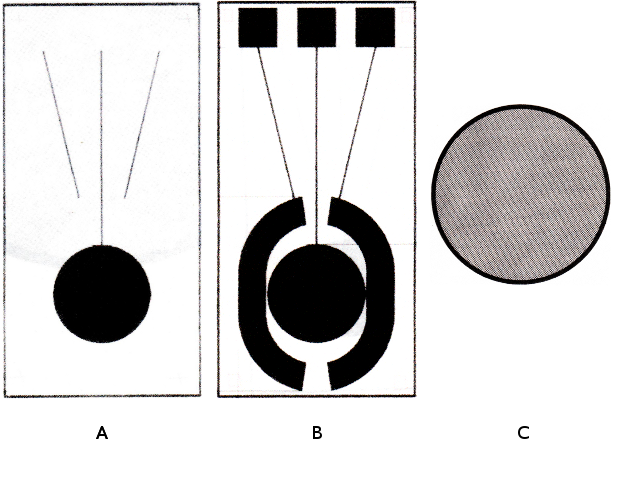
\includegraphics[width=3.5in]{../figures/stencils.png}
\end{center}
\caption{Stencils for lithography. {\bf A} is for the protective layer of resist. {\bf B} is the metal layer stencil. {\bf C} is a closeup of the diamond pattern on the active area.}
\end{figure}
